\documentclass[a4paper,10pt]{article}

\usepackage{tabularx} % extra features for tabular environment
\usepackage{amsmath}  % improve math presentation
\usepackage{graphicx} % takes care of graphic including machinery
\usepackage[margin=1in,letterpaper]{geometry} % decreases margins
\usepackage{cite} % takes care of citations
\usepackage[final]{hyperref} % adds hyper links inside the generated pdf file
\usepackage{ctex}
\usepackage{titlesec}
%\usepackage{CJKutf8, CJK}
\usepackage{makecell}                 % 三线表-竖线
\usepackage{booktabs}                 % 三线表-短细横线
% \usepackage{natbib}
\usepackage{graphicx}				  % 表格单元格逆时针
\usepackage{multirow}				  % 合并单元格
\usepackage{array}
\usepackage{amssymb}				  % 勾
\usepackage{amsmath}
\usepackage{longtable}                % 导入 longtable 宏包,表格自动换行
\usepackage{caption}
\usepackage{subcaption}               % 设置子图
\usepackage{color}					  % 文本颜色包
\usepackage{xcolor}
\usepackage{bbm}					  % 输入指示函数
\usepackage{tablefootnote}			  % 表格注释
\usepackage{pythonhighlight}
\usepackage{fancyhdr}
\usepackage{lastpage}
\pagestyle{fancy}
\fancyhf{}
\fancyhead{}
\fancyfoot{}
\fancyhead[R]{\small Page \thepage\ of \pageref*{LastPage}}
\fancyhead[L]{\small Report}

\usepackage{listings}                 % 导入代码块
\usepackage{xcolor}
\lstset{
	numbers=left, 
	tabsize=1,
	columns=flexible, 
	numberstyle=  \small, 
	keywordstyle= \color{ blue!70},
	commentstyle= \color{red!50!green!50!blue!50}, 
	frame=shadowbox, % 阴影效果
	rulesepcolor= \color{ red!20!green!20!blue!20} ,
	escapeinside=``, % 英文分号中可写入中文
	xleftmargin=2em,
	xrightmargin=2em, 
	aboveskip=1em,
} 

\hypersetup{
	colorlinks=true,       % false: boxed links; true: colored links
	linkcolor=blue,        % color of internal links
	citecolor=blue,        % color of links to bibliography
	filecolor=magenta,     % color of file links
	urlcolor=blue         
}
%++++++++++++++++++++++++++++++++++++++++
\titleformat{\section}{\Large\bfseries\songti}{\thesection}{1em}{}
\titleformat{\subsection}{\large\bfseries\songti}{\thesubsection}{1em}{}
\titleformat{\subsubsection}{\normalsize\bfseries\songti}{\thesubsubsection}{1em}{}
\titleformat{\paragraph}{\small\bfseries\songti}{\paragraph}{1em}{}
\titleformat{\subparagraph}{\footnotesize\bfseries\songti}{\subparagraph}{1em}{}

\begin{document}
	
	
	\title{\songti \zihao{4}Unity VR 项目开发进度}
%	\author{\textrm{Ku Jui}}
	\date{\textrm{October 2023}}
	\maketitle
	
	\renewcommand{\figurename}{Figure} % 可以重新定义abstract,因为ctex会覆盖thebibliography
	% 	\begin{abstract}
		%		In this experiment we studied a very important physical effect by measuring the
		%		dependence of a quantity $V$ of the quantity $X$ for two different sample
		%		temperatures.  Our experimental measurements confirmed the quadratic dependence
		%		$V = kX^2$ predicted by Someone's first law. The value of the mystery parameter
		%		$k = 15.4\pm 0.5$~s was extracted from the fit. This value is
		%		not consistent with the theoretically predicted $k_{theory}=17.34$~s. We attribute %this
		%		discrepancy to low efficiency of our $V$-detector.
		%	\end{abstract}
	\renewcommand{\contentsname}{Contents}
	\renewcommand{\tablename}{Table}
	\tableofcontents  % 自动生成目录
		
	\section{开发进度}
		
		\subsection{已知问题}
		
		\begin{figure}[htbp] 
			% read manual to see what [ht] means and for other possible options
			\centering 
			% 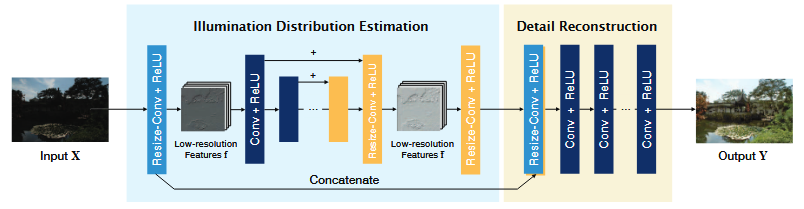
\includegraphics[width=0.8\columnwidth]{GLADNet}
			
			\begin{subfigure}{0.23\textwidth}
				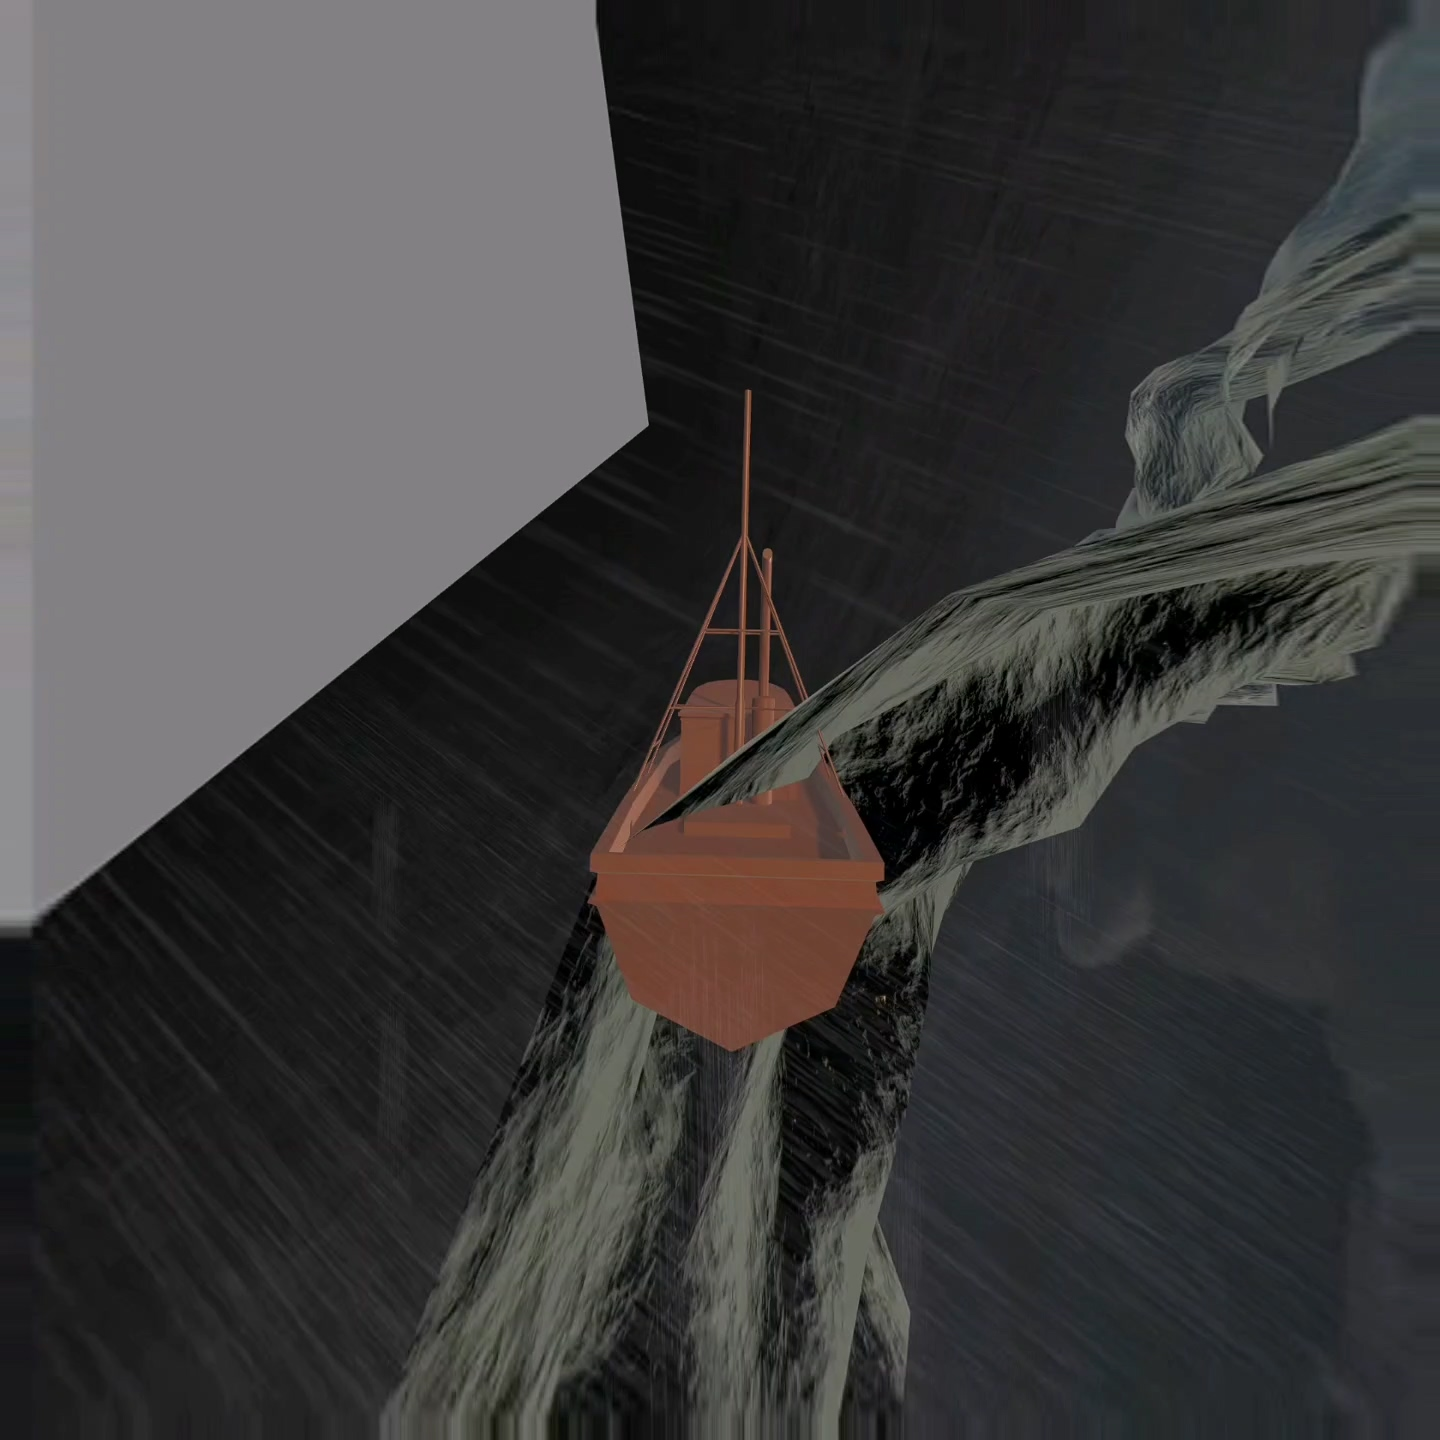
\includegraphics[width=\linewidth]{picture/bug1-shipwreck-storm}
				\captionsetup{font=scriptsize}
				\caption{shipwreck1}
				\label{fig: bug1-shipwreck-storm}
			\end{subfigure}
			\begin{subfigure}{0.23\textwidth}
				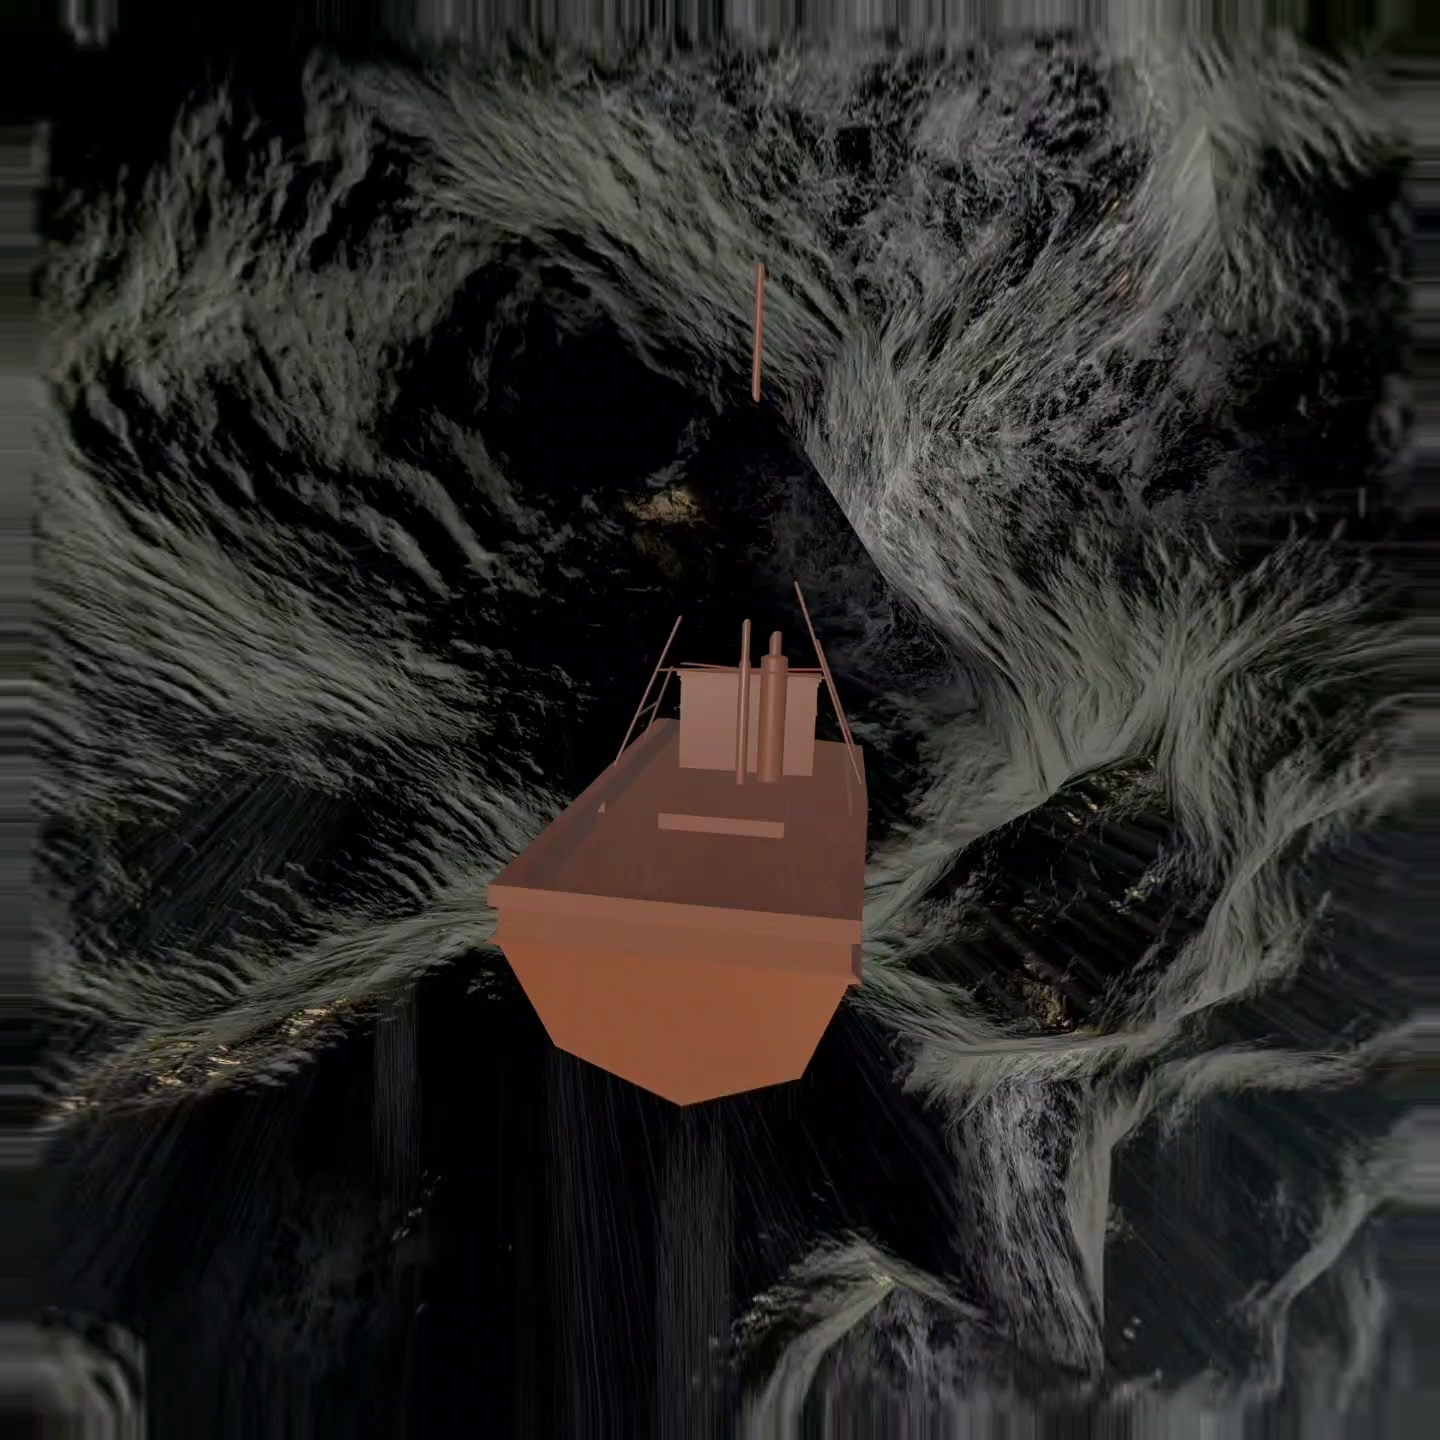
\includegraphics[width=\linewidth]{picture/bug2-shipwreck-storm}
				\captionsetup{font=scriptsize}
				\caption{shipwreck2}
				\label{fig: bug2-shipwreck-storm}
			\end{subfigure}
			\begin{subfigure}{0.23\textwidth}
				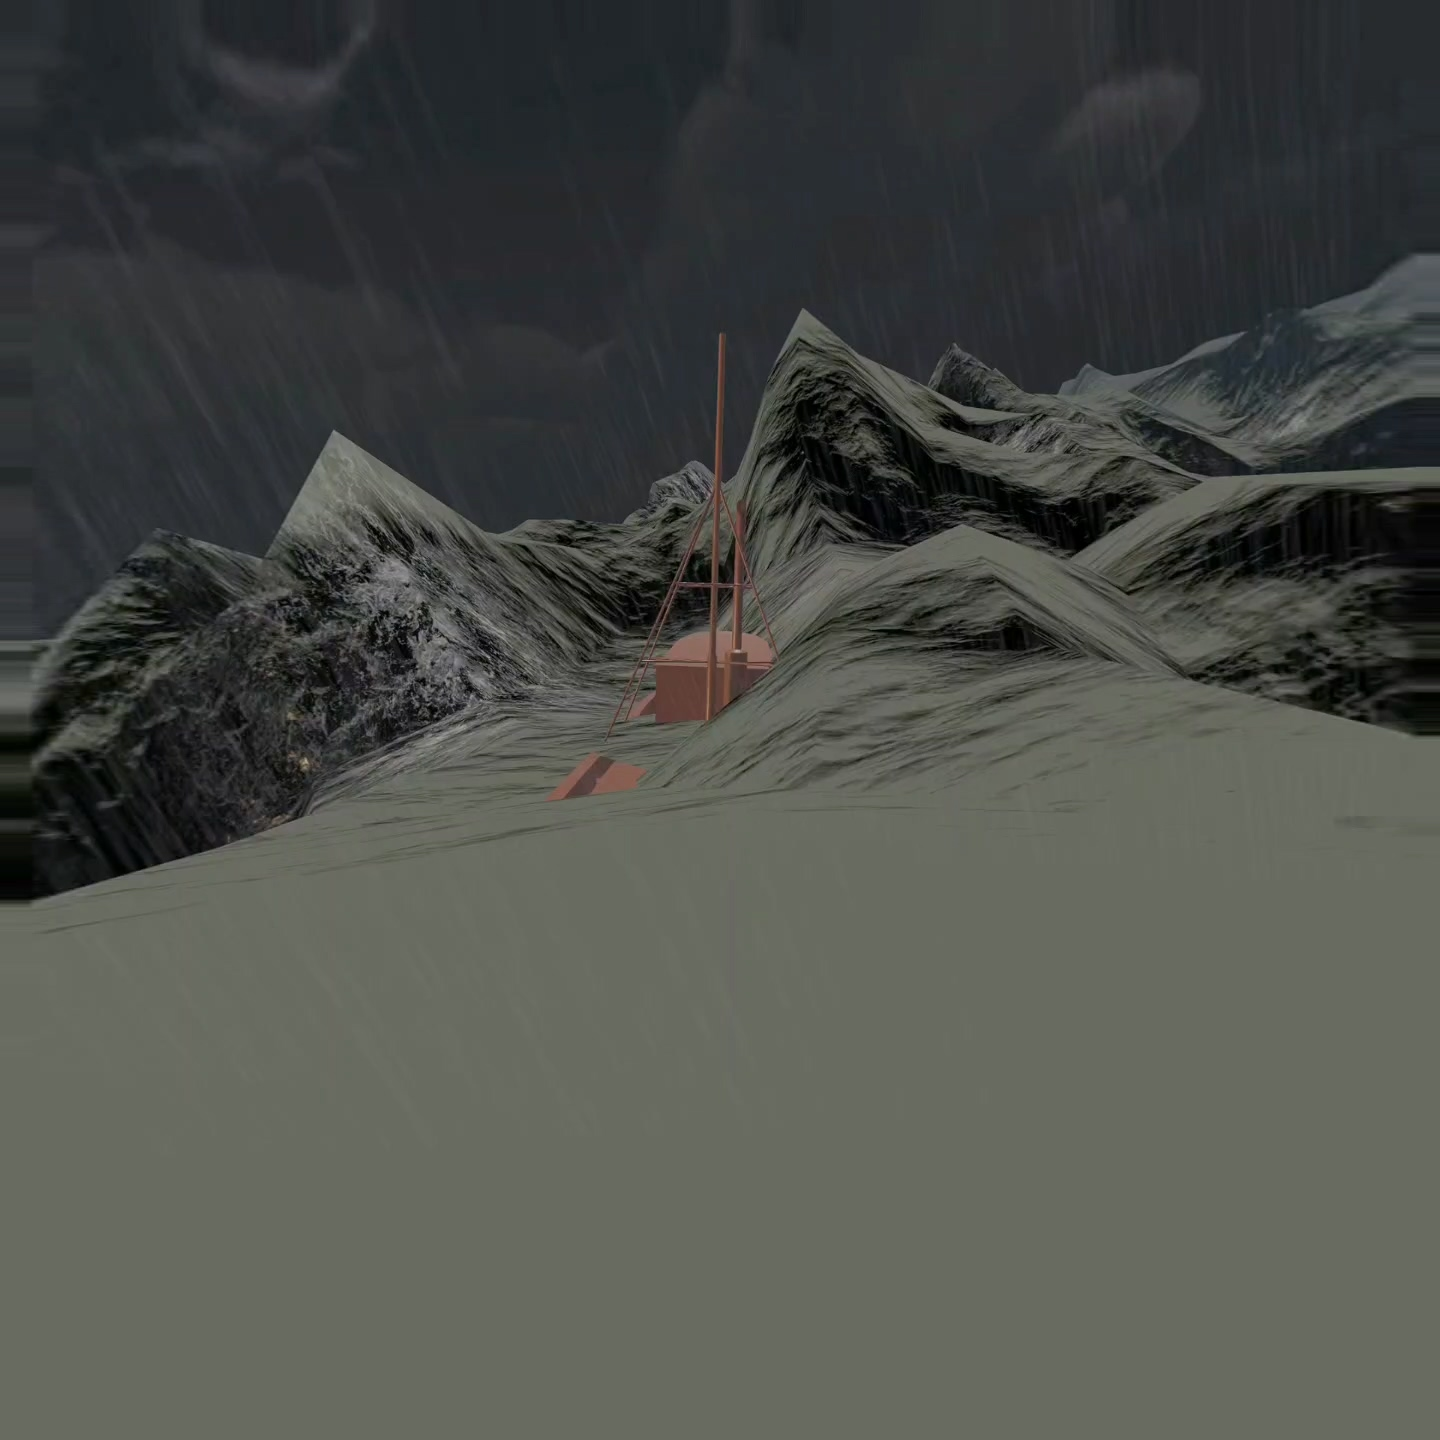
\includegraphics[width=\linewidth]{picture/bug3-modeltwist-storm}
				\captionsetup{font=scriptsize}
				\caption{model twist}
				\label{fig: bug3-modeltwist-storm}
			\end{subfigure}
			\begin{subfigure}{0.23\textwidth}
				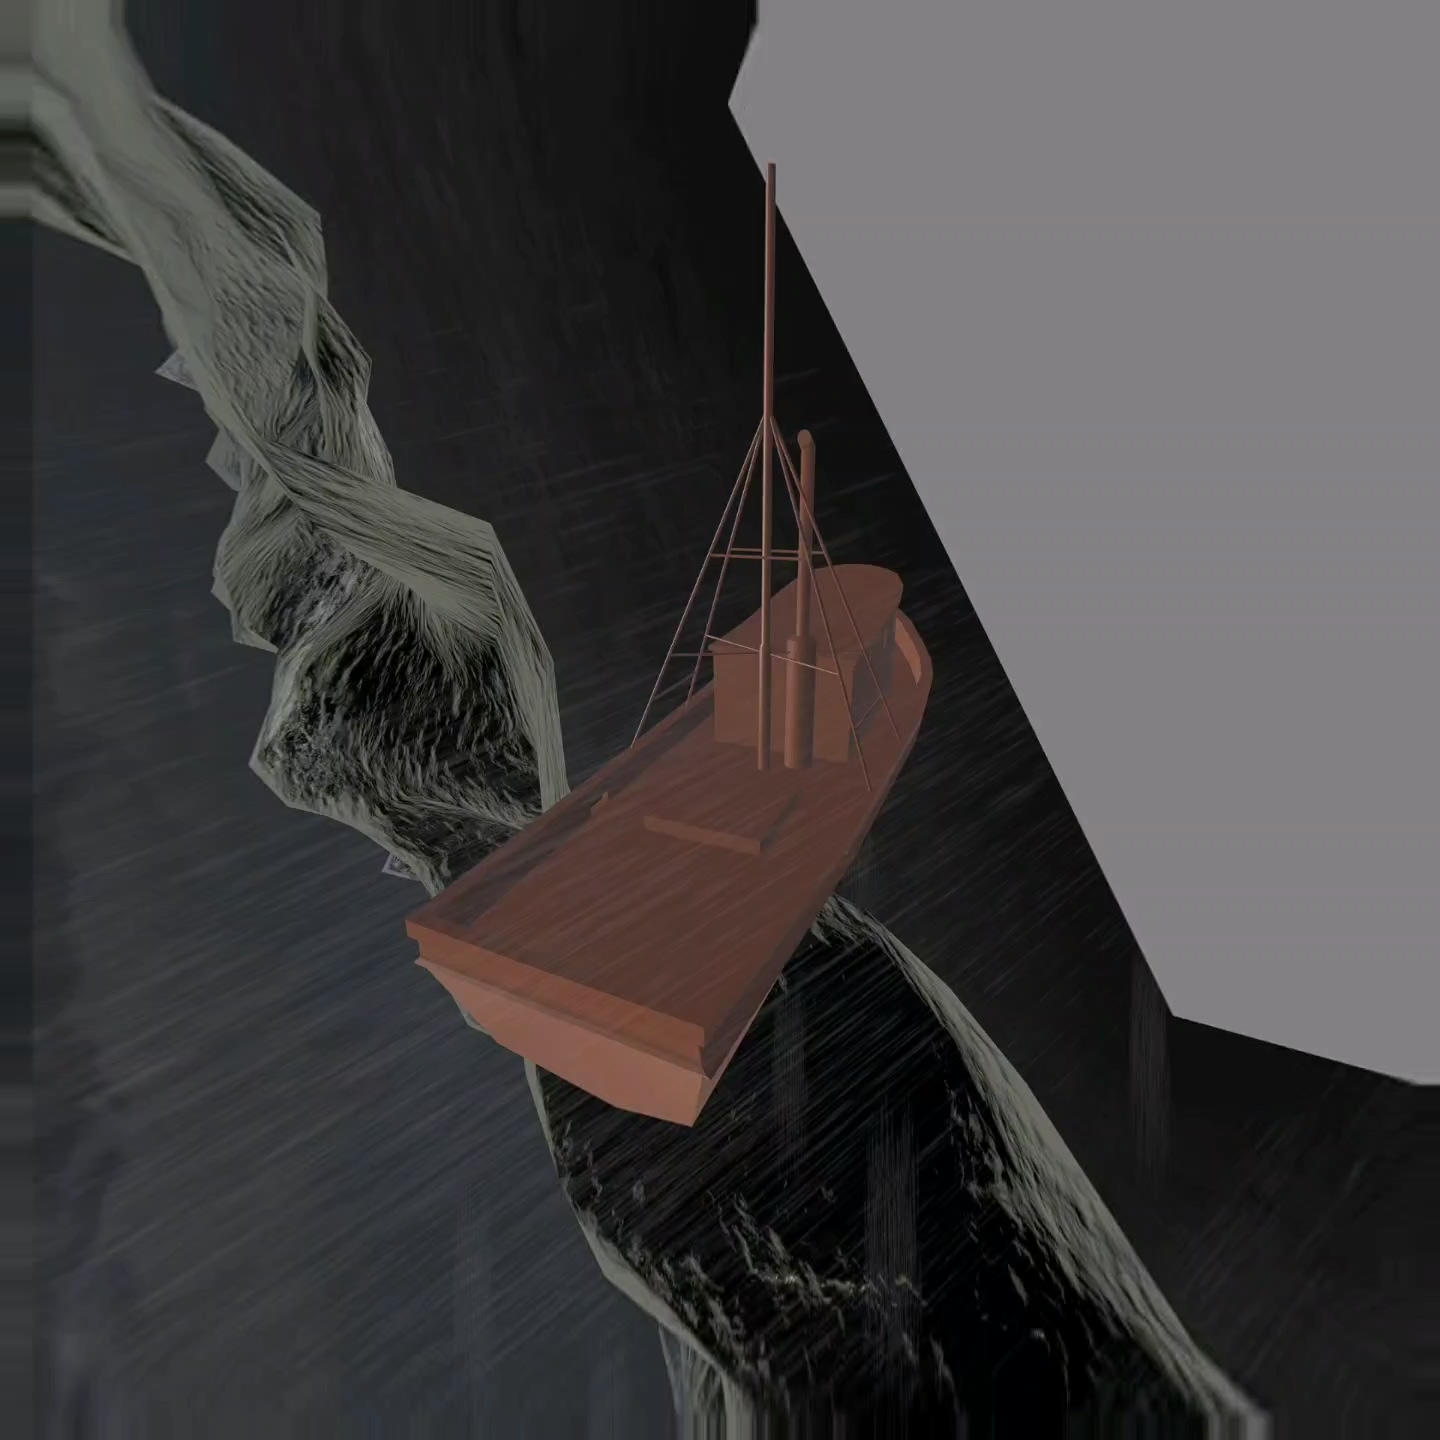
\includegraphics[width=\linewidth]{picture/bug4-shipwreck-storm}
				\captionsetup{font=scriptsize}
				\caption{shipwreck3}
				\label{fig: bug4-shipwreck-storm}
			\end{subfigure} \\
			
			\begin{subfigure}{0.23\textwidth}
				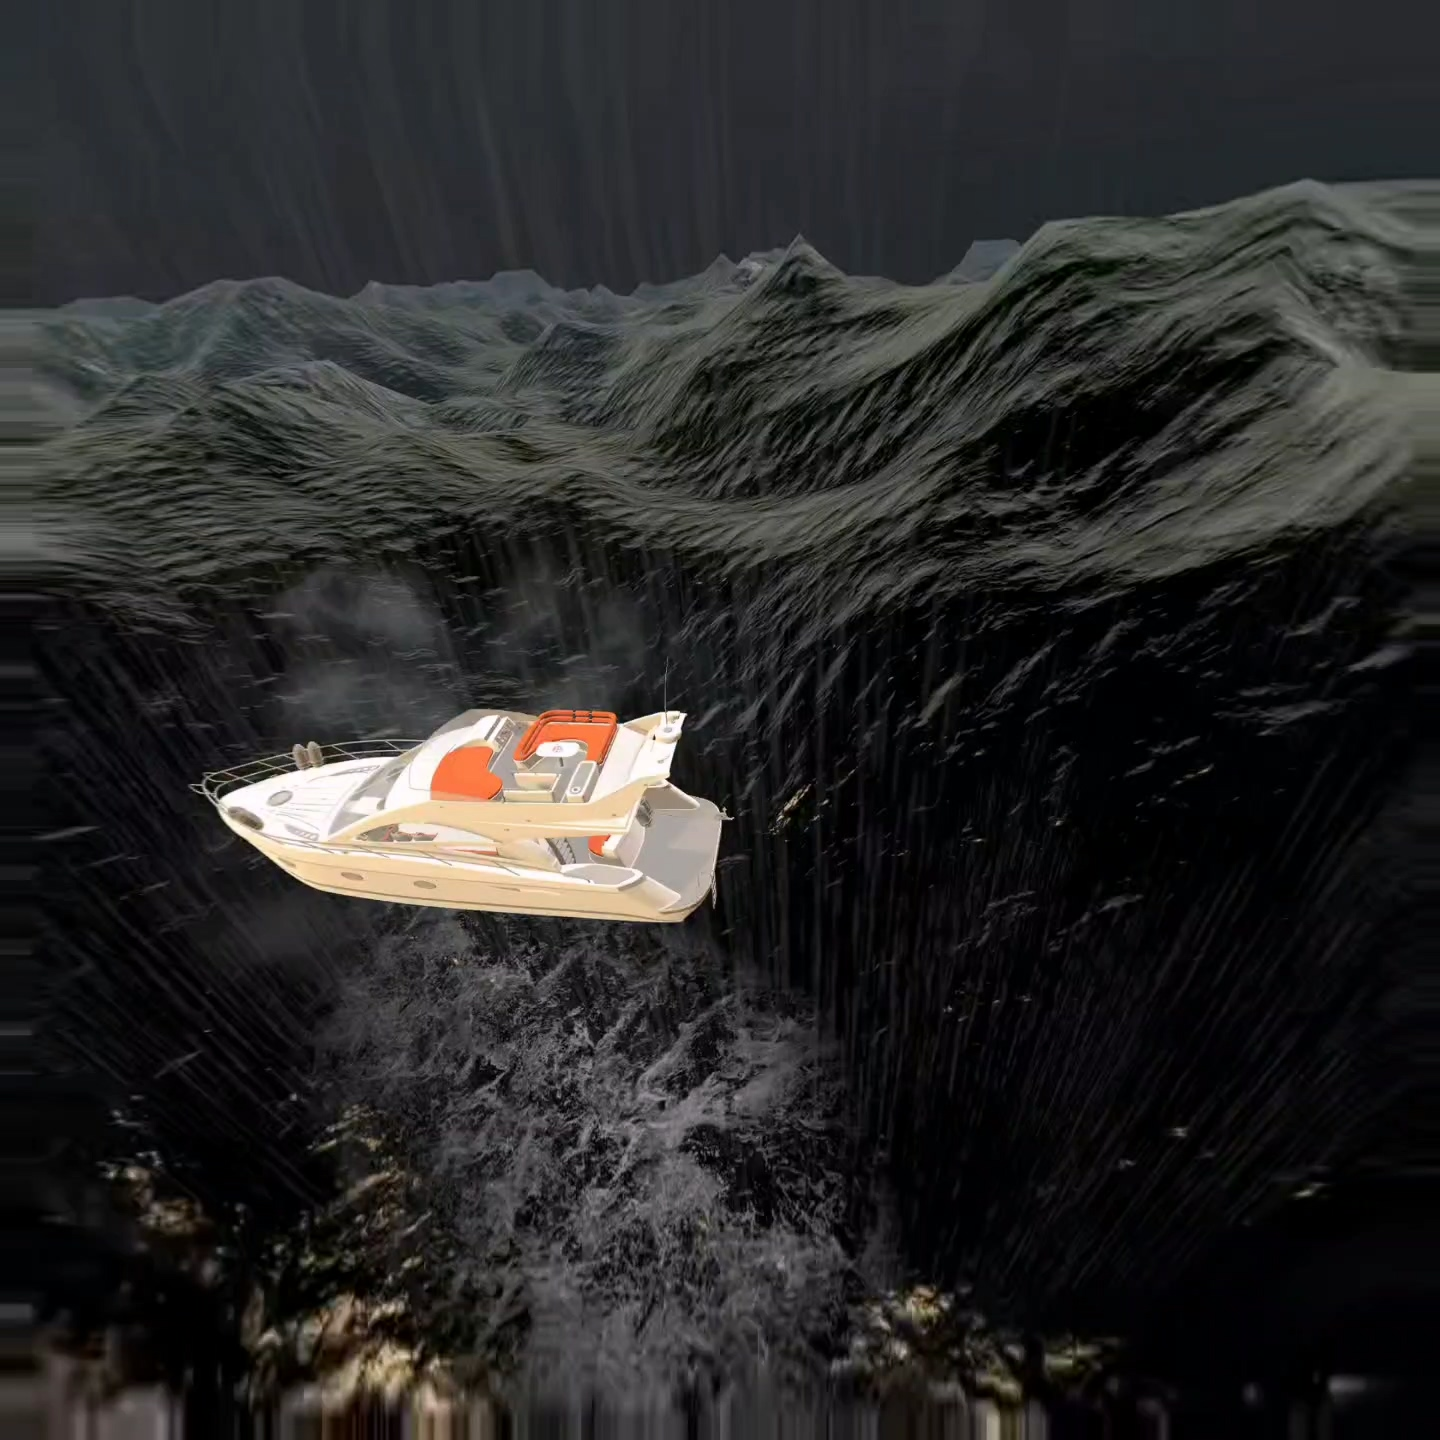
\includegraphics[width=\linewidth]{picture/bug5-modeltwist-storm}
				\captionsetup{font=scriptsize}
				\caption{model twist}
				\label{fig: bug5-modeltwist-storm}
			\end{subfigure}
			\begin{subfigure}{0.23\textwidth}
				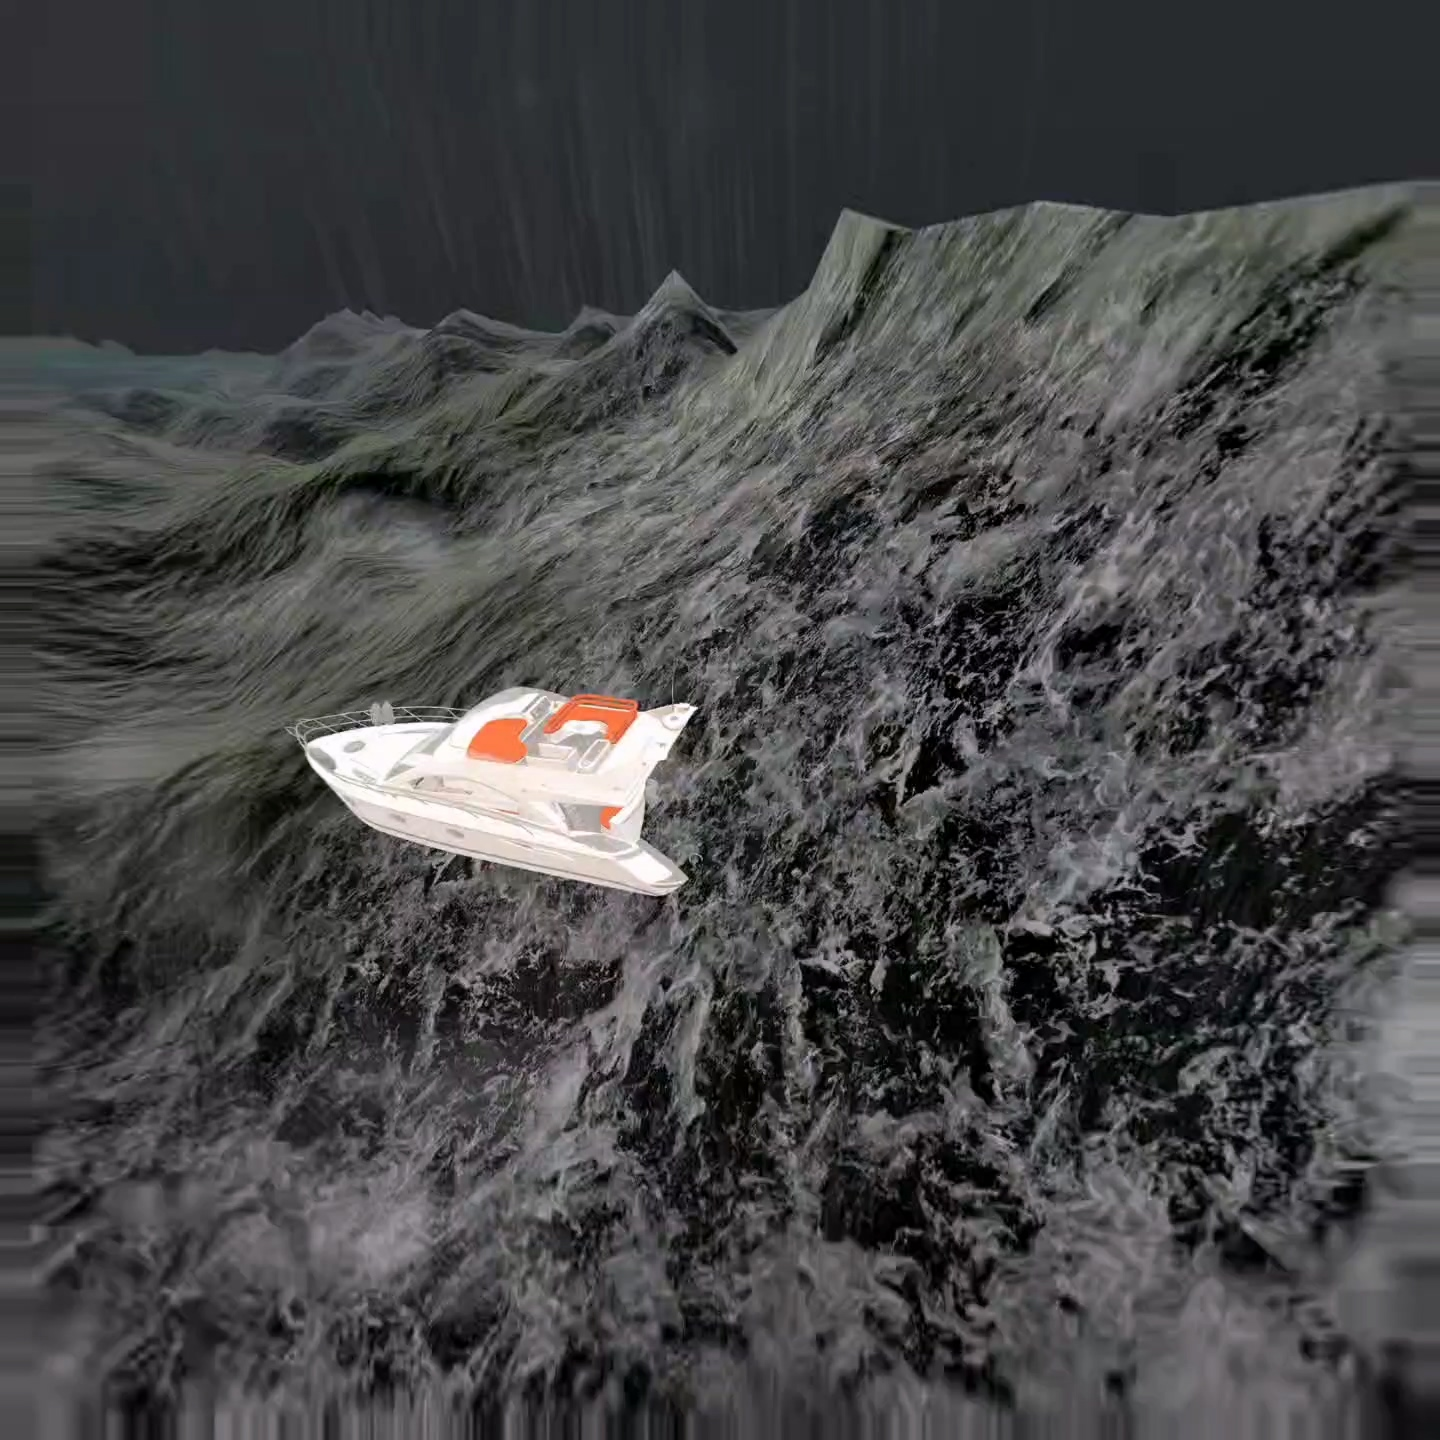
\includegraphics[width=\linewidth]{picture/bug6-controlfailure}
				\captionsetup{font=scriptsize}
				\caption{control failure}
				\label{fig: bug6-controlfailure}
			\end{subfigure}
			\begin{subfigure}{0.23\textwidth}
				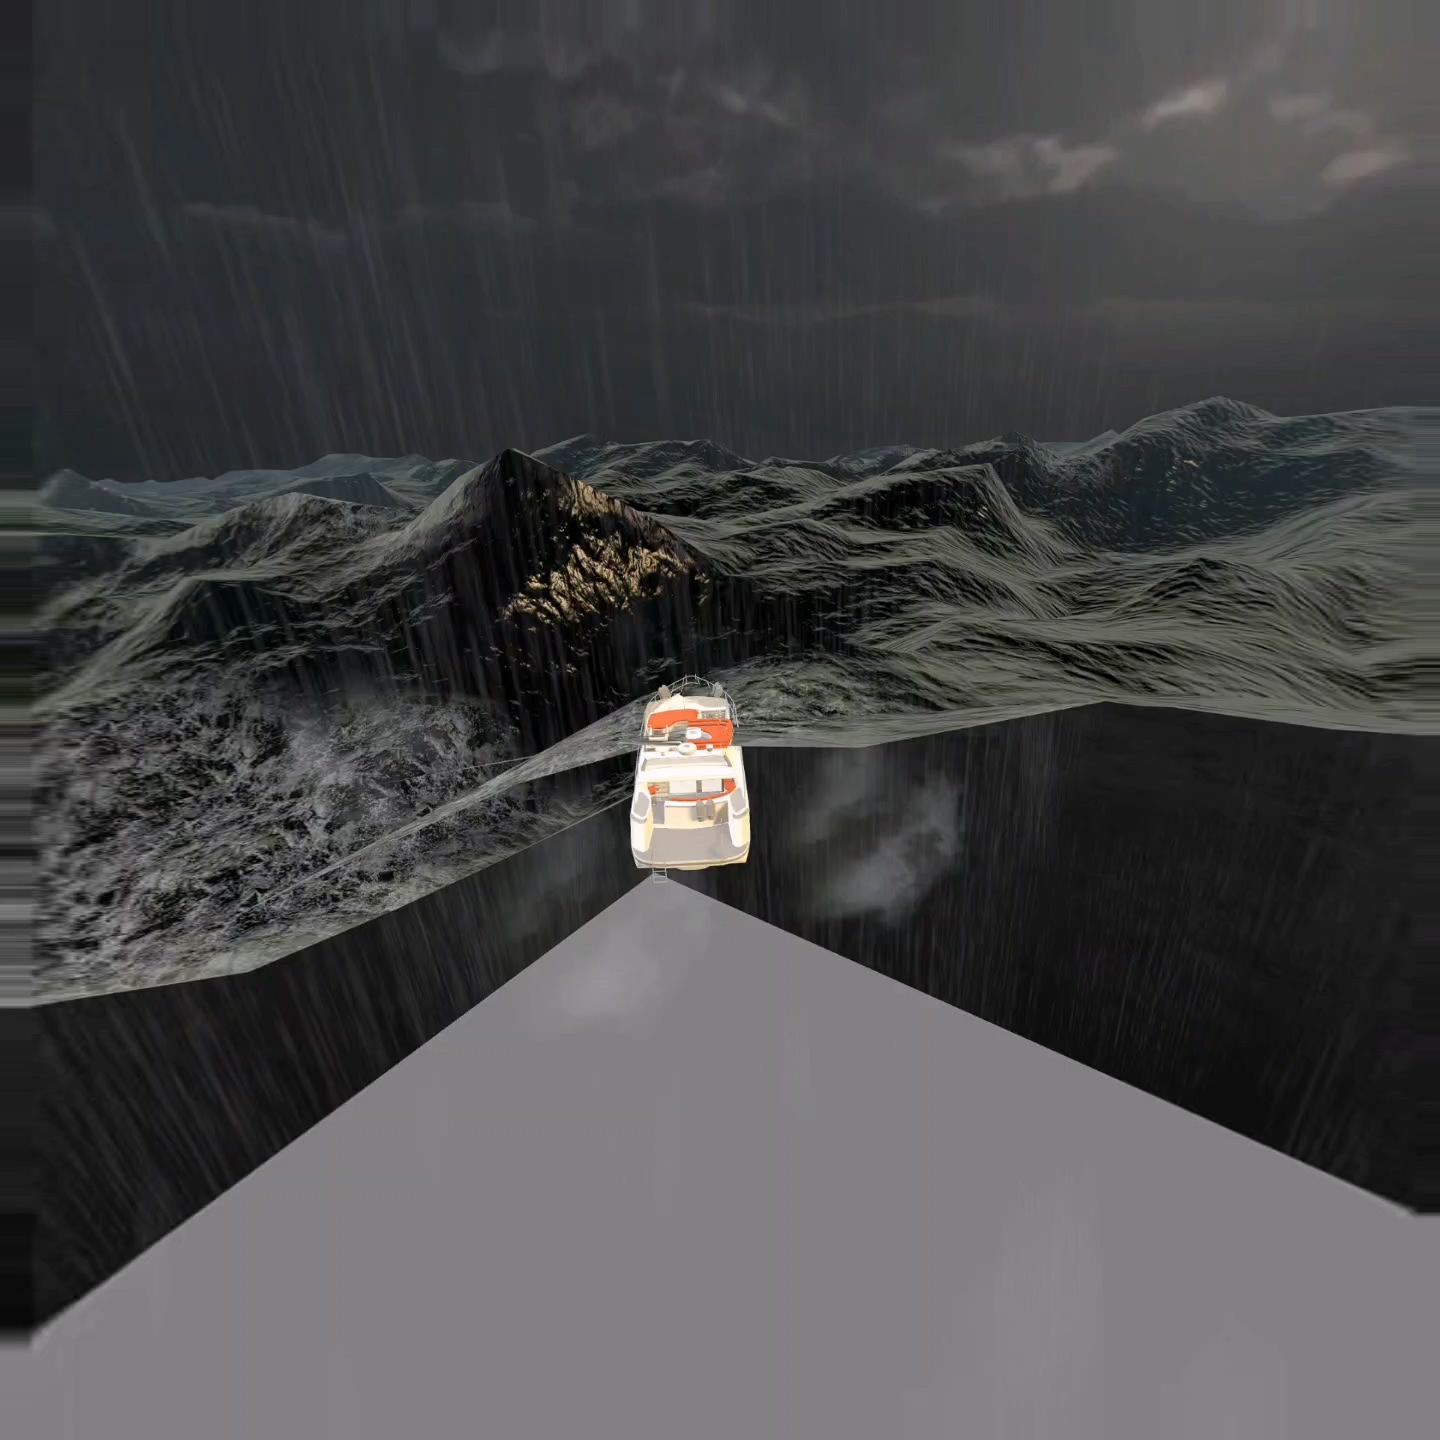
\includegraphics[width=\linewidth]{picture/bug7-modeltwist-storm}
				\captionsetup{font=scriptsize}
				\caption{model twist}
				\label{fig: bug7-modeltwist-storm}
			\end{subfigure}
			\begin{subfigure}{0.23\textwidth}
				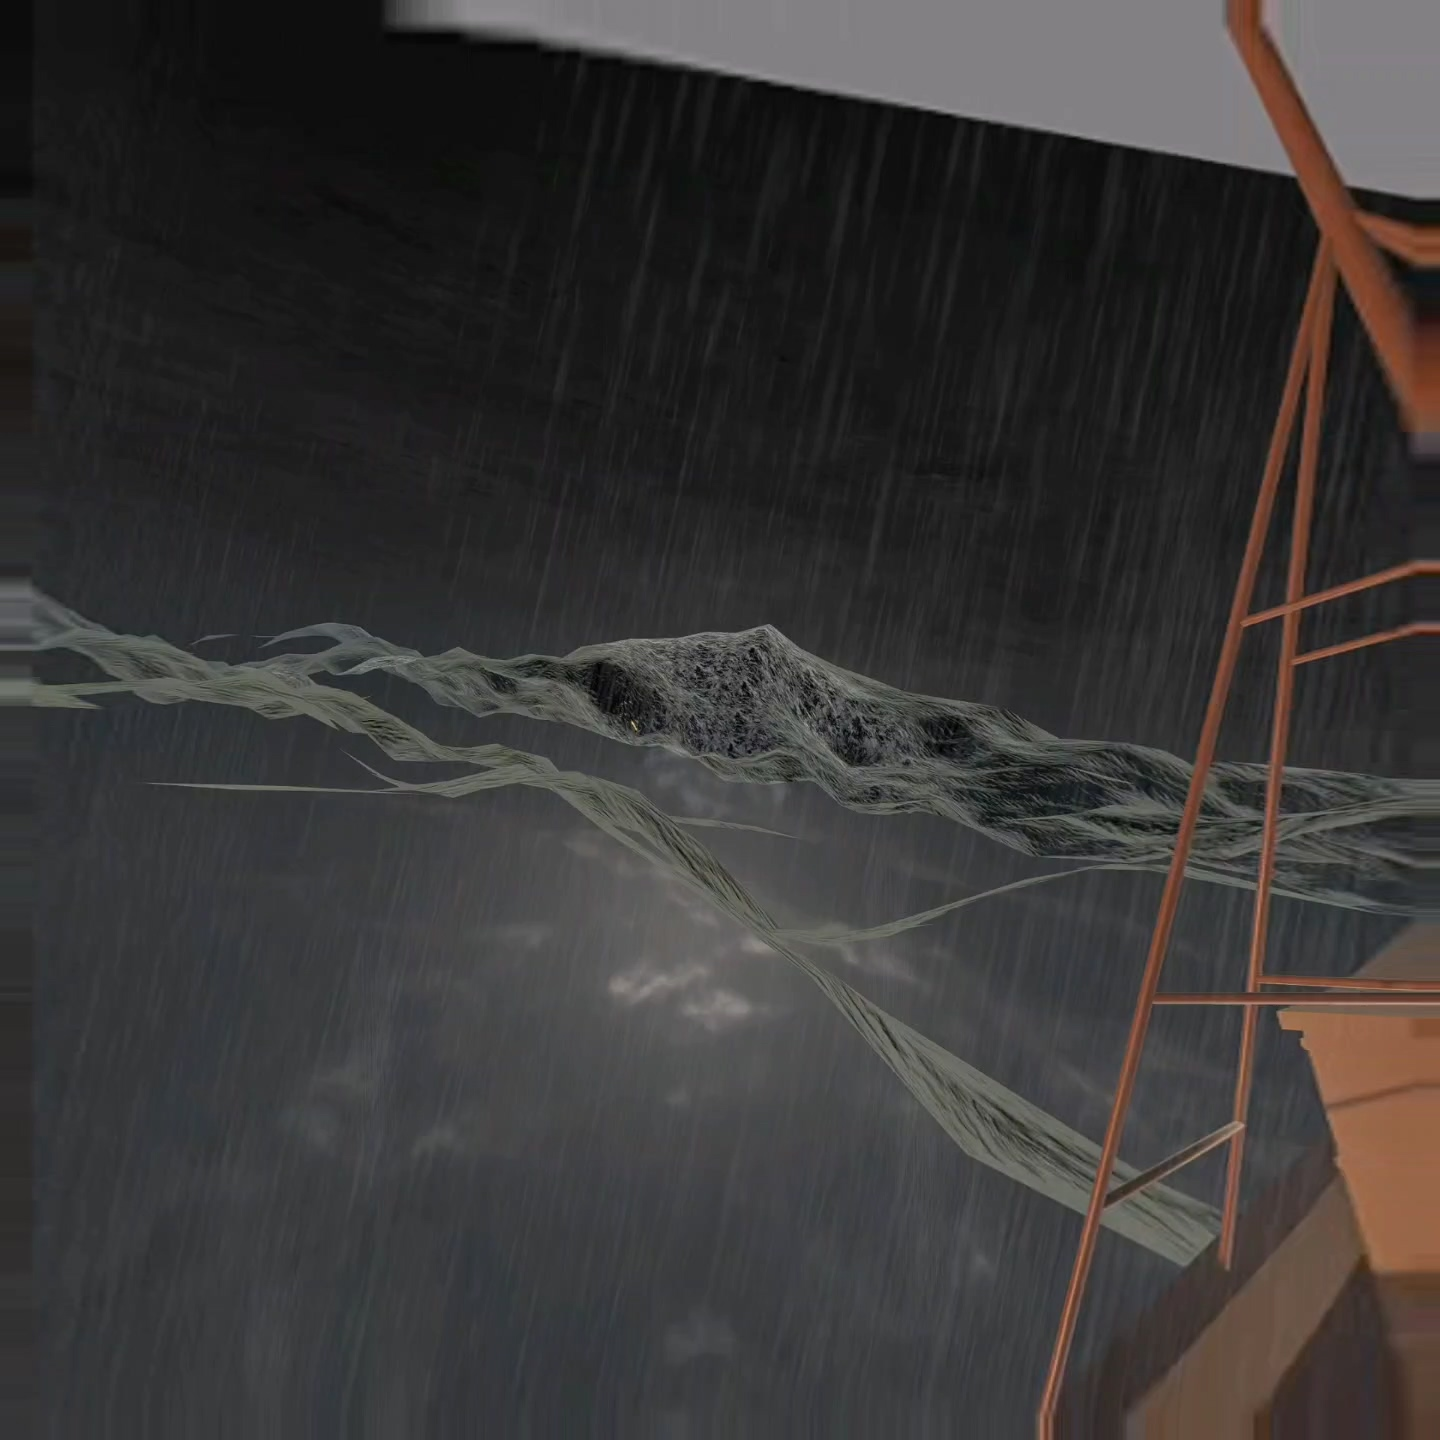
\includegraphics[width=\linewidth]{picture/bug8-shipwreck-storm}
				\captionsetup{font=scriptsize}
				\caption{shipwreck}
				\label{fig: bug8-shipwreck-storm}
			\end{subfigure}
			
			\captionsetup{font=scriptsize}
			\caption{
				\label{fig: bug}	
				目前已知游戏bug				
			}
		\end{figure}

		\paragraph{bug1:雨天船只翻船}
		
		在雨天天气下,选择模型2船只,如 Fig. \ref{fig: bug1-shipwreck-storm}, Fig . \ref{fig: bug2-shipwreck-storm}, Fig .\ref{fig: bug4-shipwreck-storm} 和 Fig. \ref{fig: bug8-shipwreck-storm} 所示,船只会翻入海面(海面翻转)或是丢失船只姿态。

		\paragraph{bug2:海面缺失}
		
		在雨天天气下,选择模型2船只,如 Fig. \ref{fig: bug3-modeltwist-storm}所示,会出现船只与海面的穿模现象。
		
		\paragraph{bug3: 船只操控故障}
		
		在雨天天气和冰雹天气下,选择模型1船只,如 Fig. \ref{fig: bug5-modeltwist-storm} 和 Fig. \ref{fig: bug6-controlfailure} 所示,船只会受到右手柄方向仪的控制,表现为疯狂向左旋转,无法控制船只行驶。
		
		\paragraph{bug4:船只模型故障}

		在雨天天气下,模型1船只并不会随着海浪而摇摆,表现为只能在固定的平面移动,可以随意穿越海浪,如 Fig. \ref{fig: bug6-controlfailure} 所示。因模型不兼容此天气的海浪插件所致。
		
		\paragraph{bug5:海浪缺失}
		
		在雨天天气下,模型1船只并不会随着海浪而摇摆,开启船只之后,可以随意穿越海浪,会出现海浪缺失,如 Fig. \ref{fig: bug7-modeltwist-storm} 所示。因模型不兼容此天气的海浪插件所致。
		
	%	\section{Analysis}
	
	%	In this section you will need to show your experimental results. Use tables and
	%	graphs when it is possible. Table~\ref{tbl:bins} is an example.
	
	%	\begin{table}[ht]
		%		\begin{center}
			%			\caption{Every table needs a caption.}
			%			\label{tbl:bins} % spaces are big no-no withing labels
			%			\begin{tabular}{|ccc|} 
				%				\hline
				%				\multicolumn{1}{|c}{$x$ (m)} & \multicolumn{1}{c|}{$V$ (V)} & \multicolumn{1}{c|}{$V$ (V)} \\
				%				\hline
				%				0.0044151 &   0.0030871 &   0.0030871\\
				%				0.0021633 &   0.0021343 &   0.0030871\\
				%				0.0003600 &   0.0018642 &   0.0030871\\
				%				0.0023831 &   0.0013287 &   0.0030871\\
				%				\hline
				%			\end{tabular}
			%		\end{center}
		%	\end{table}
	%	
	%	Analysis of equation~\ref{eq:aperp} shows ...
	%	
	%	Note: this section can be integrated with the previous one as long as you
	%	address the issue. Here explain how you determine uncertainties for different
	%	measured values. Suppose that in the experiment you make a series of
	%	measurements of a resistance of the wire $R$ for different applied voltages
	%	$V$, then you calculate the temperature from the resistance using a known
	%	equation and make a plot  temperature vs. voltage squared. Again suppose that
	%	this dependence is expected to be linear~\cite{Cyr}, and the proportionality coefficient
	%	is extracted from the graph. Then what you need to explain is that for the
	%	resistance and the voltage the uncertainties are instrumental (since each
	%	measurements in done only once), and they are $\dots$. Then give an equation
	%	for calculating the uncertainty of the temperature from the resistance
	%	uncertainty. Finally explain how the uncertainty of the slop of the graph was
	%	found (computer fitting, graphical method, \emph{etc}.)
	%	
	%	If in the process of data analysis you found any noticeable systematic
	%	error(s), you have to explain them in this section of the report.
	%	
	%	It is also recommended to plot the data graphically to efficiently illustrate
	%	any points of discussion. For example, it is easy to conclude that the
	%	experiment and theory match each other rather well if you look at
	%	Fig.~\ref{fig:samplesetup} and Fig.~\ref{fig:exp_plots}.
	%	
	%	\begin{figure}[ht] 
		%		\centering
		%		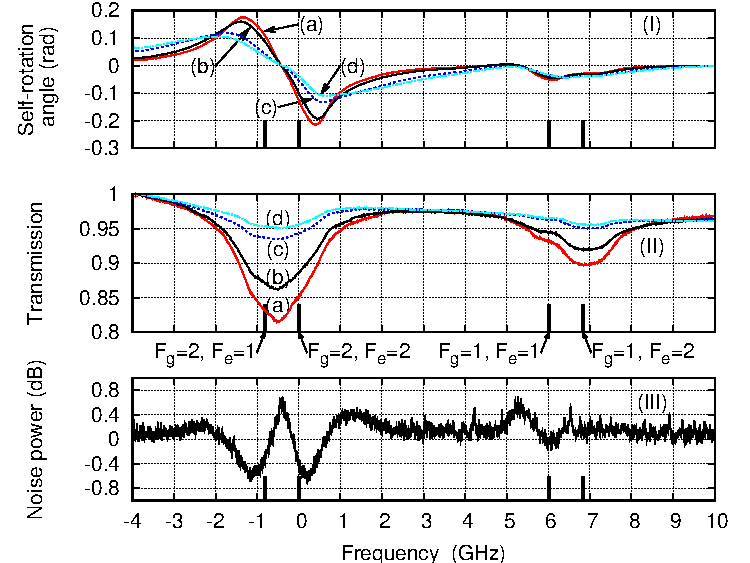
\includegraphics[width=0.5\columnwidth]{sr_squeezing_vs_detuning}
		%		
		%		% some figures do not need to be too wide
		%		\caption{
			%			\label{fig:exp_plots}  
			%			Every plot must have axes labeled.
			%		}
		%	\end{figure}
	
	
	%	\section{Conclusions}
	%	Here you briefly summarize your findings.
	
	%++++++++++++++++++++++++++++++++++++++++
	% References section will be created automatically 
	% with inclusion of "thebibliography" environment
	% as it shown below. See text starting with line
	% \begin{thebibliography}{99}
		% Note: with this approach it is YOUR responsibility to put them in order
		% of appearance.
		
%		\renewcommand{\refname}{References}
		
		
		%	\begin{thebibliography}{00}
			
			%		\bibitem{b1}\label{cite:b1}
			%		W. Wang, C. Wei, W. Yang and J. Liu, "GLADNet: Low-Light Enhancement Network with Global Awareness," 2018 13th IEEE International Conference on Automatic Face \& Gesture Recognition (FG 2018), Xi'an, China, 2018, pp. 751-755, DOI: 10.1109/FG.2018.00118.
			
			%		\bibitem{b2}\label{cite:b2}
			%		A.\ Mahajan, K.\ Somaraj and M. Sameer, "Adopting Artificial Intelligence Powered ConvNet To Detect Epileptic Seizures," 2020 IEEE-EMBS Conference on Biomedical Engineering and Sciences (IECBES), Langkawi Island, Malaysia, 2021, pp. 427-432, DOI: 10.1109/IECBES48179.2021.9398832.
			
			%		\bibitem{Cyr}
			%		N.\ Cyr, M.\ T$\hat{e}$tu, and M.\ Breton,
			% "All-optical microwave frequency standard: a proposal,"
			%		IEEE Trans.\ Instrum.\ Meas.\ \textbf{42}, 640 (1993).
			
			
			
			%	\end{thebibliography}
		
%		\bibliographystyle{unsrt}
%		\bibliography{reference}
		
		
	\end{document}
